\documentclass[12pt]{article}
\usepackage{inputenc}
\usepackage[top=1in, bottom=1in, left=1in, right=1in]{geometry}
\usepackage{setspace}
\usepackage{parskip}
\setcounter{secnumdepth}{1}
\pagestyle{plain}
\usepackage{graphicx}
%\usepackage{fontspec}
%\setmainfont{Georgia}
\setlength{\parindent}{0 cm}
\usepackage[section]{placeins}


\usepackage[compact]{titlesec}  
\usepackage{amssymb}
\usepackage{amsmath}
\newcommand\numberthis{\addtocounter{equation}{1}\tag{\theequation}}
\titlespacing{\section}{0pt}{0pt}{0pt}
\usepackage{changepage}
\newenvironment{myenv}{\begin{adjustwidth}{1cm}{}}{\end{adjustwidth}}

\begin{document}
% Manual Heading
{\raggedleft{}Gabriel Griggs} \\
Professor Mark Alber \\
Nonlinear Dynamical Systems: ACMS 403630 --- 01 \\
Thursday, January 30th 2014\\
Homework 1
\section*{Question 1}
\begin{myenv}
\textbf{Question:} Consider a differential equation $ \dot{x} = f(x) = ax - x^3$ for some $a \in \mathbb{R}$. Determine fixed points and their stability for cases where $a$ is positive, negative, and zero.

\textbf{Answer:} In order to determine the fixed points, we must set $ f(\bar{x}) = 0 $ and solve for $ \bar{x} $. This yields:
\begin{align*}
f(\bar{x}) = 0 = a\bar{x}-\bar{x}^3 = x(a-\bar{x}^2)
\end{align*}
\begin{align*}
\bar{x} = 0, \pm\sqrt{a}
\end{align*}

Thus, our fixed points are going to be located at $\bar{x} = 0$ and $\pm\sqrt{a}$. In order to determine the stability at each of these points for the three cases of a, we will graph them using $a = 4, a = 0$ and $a = -4$ as representative cases.

Our first case $ a = 4 $, represents the case where $ a > 0 $. Seen in the graphs below, this scenario yields stable fixed points at $ \pm\sqrt(a) $ and an unstable node at $a = 0$. For $a = 0$, we have one stable node at the origin. Finally, for the $ a < 0 $ case, we use $ a = -4 $ as a proxy. This graph reveals a similar one to the $ a = 0 $ case in that there is a stable node at the origin.

\begin{figure} [H]
    \centering
    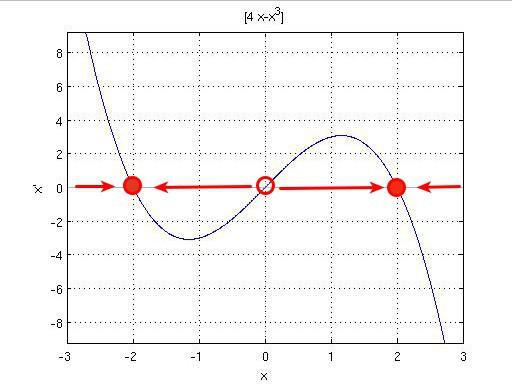
\includegraphics[width=0.8\textwidth]{a41}
    \caption{$ a > 0$ represented by $ a = 4 $}
    \label{figure:a1}
\end{figure}

\begin{figure} [H]
    \centering
    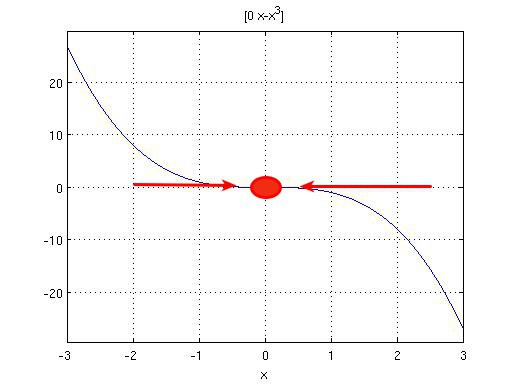
\includegraphics[width=0.8\textwidth]{a0}
    \caption{ $ a = 0$}
    \label{figure:a0}
\end{figure}

\begin{figure} [H]
    \centering
    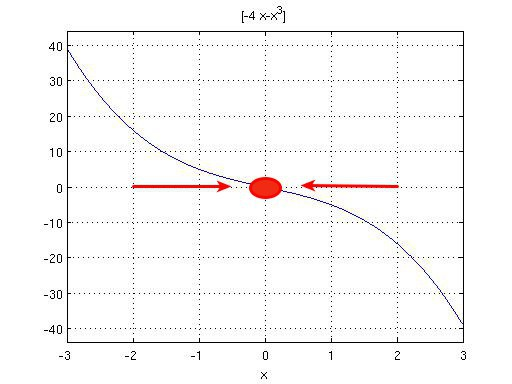
\includegraphics[width=0.8\textwidth]{anegative4}
    \caption{ $ a = 0$}
    \label{figure:a0}
\end{figure}

\end{myenv}

\section*{Question 2}
\begin{myenv}
\textbf{Question:} Find fixed points and sketch nullclines, vector field and plausible phase portrait of the system:
\begin{alignat*}{3}
\dot{x} &= x(x-y) &= f(x,y) \\
\dot{y} &= y(2x-y) &= g(x,y)
\end{alignat*}


\textbf{Answer:} In order to find the fixed points, we need to find $(\bar{x},\bar{y})$ such that $f(\bar{x},\bar{y}) = 0$ and $g(\bar{x},\bar{y}) = 0$. Thus, the only fixed point occurs at $(0,0)$.

The Jacobian matrix at a general point in this system is given as:
\begin{align*}
	J &= 
	\begin{Bmatrix}
	2x-y & -x \\
	2y & -2y + 2x
	\end{Bmatrix}
\end{align*}

Evaluating the Jacobian at the fixed point $(0,0)$ yields:
\begin{align*}
	J &= 
	\begin{Bmatrix}
	0 & 0 \\
	0 & 0
	\end{Bmatrix}, 	&\Lambda^2 &= 0,	&\Lambda &= 0, &det &= 0, &trace &= 0
\end{align*}
\end{myenv}

This analysis tells us that linearization of our system predicts a center at $(0,0)$. However, by looking at a graph of the vector field and the null clines (at lines $x = 0, y = 0,$ and $y = 2x$), reveals that there is not a center (or at least, not a typical center). This graph can be seen below. The fact that this is not a typical center becomes even clearer when we look at the vector field graph with possible solutions overlaid. It appears that initial conditions in the 1st and 3rd quadrants return to the origin, while initial solutions in the 2nd and 4th quadrant go to infinity. This graph can be seen, with the caption ``Phase Portrait'', below.



\begin{figure} [H]
    \centering
    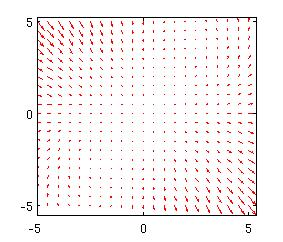
\includegraphics[width=0.8\textwidth]{Question2_VectorField}
    \caption{ Vector Field and Nullclines}
    \label{figure:a0}
\end{figure}


\begin{figure} [H]
    \centering
    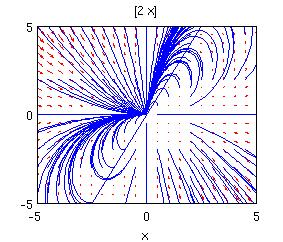
\includegraphics[width=0.8\textwidth]{Question2_PhasePortrait}
    \caption{ Phase Portrait}
    \label{figure:a0}
\end{figure}




\end{document}

